\documentclass{article}

\usepackage{polski}
\usepackage{amsmath, array}
\usepackage{graphicx}
\usepackage{float}
\usepackage{subfig}
\usepackage{multirow}
\usepackage{enumitem}

\title{Laboratorium 4}
\author{\textbf{Łukasz Wala}\\
    \textit{AGH, Wydział Informatyki, Elektroniki i Telekomunikacji} \\
    \textit{Teoria Współbieżności 2022/23}}
\date{Kraków, \today}

\begin{document}
\maketitle

\section{Treść zadania}
Zaimplementować problem producentów i konsumentów z uwzględnieniem poniższych
zasad:
\begin{enumerate}
    \item
    Bufor o rozmiarze $2M$
    \item
    Jest $m$ producentów i $n$ konsumentów
    \item
    Producent wstawia do bufora losowa liczbę elementów (nie więcej niż $M$)
    \item
    Konsument pobiera losowa liczbę elementów (nie więcej niż $M$)
    \item
    Zaimplementować przy pomocy monitorów Javy oraz mechanizmów Java Concurrency Utilities
    \item
    Przeprowadzić porównanie wydajności (np. czas wykonywania) vs. różne parametry, zrobić wykresy i je skomentować
\end{enumerate}

\section{Implementacja - monitory}

W języku Java każdy tworzony obiekt ma przypisany do siebie monitor. Użycie słowa kluczowego
\textit{synchronized} w definicji metody sprawia, że monitor obiektu, na którym metoda jest
wywoływana, jest zablokowany na czas wykonywania, przez co pozostałe wątki chcące operować na
tym obiekcie muszą czekać na jego zwolnienie.

\begin{verbatim}
cclass Producer extends Thread {
	private Buffer buf;
    private int max;

    public Producer(Buffer buf, int max) {
        this.buf = buf;
        this.max = max;
    }

	public void run() {
      int iters = ThreadLocalRandom.current().nextInt(0, max + 1);

	  for (int i = 0; i < iters; ++i) {
		buf.put(i);
	  }
	}
}

class Consumer extends Thread {
	private Buffer buf;
    private int max;

    public Consumer(Buffer buf, int max) {
        this.buf = buf;
        this.max = max;
    }

	public void run() {
      int iters = ThreadLocalRandom.current().nextInt(0, max + 1);

	  for (int i = 0; i < iters; ++i) {
		System.out.println(buf.get());
	  }
	}
}

class Buffer {
    private List<Integer> buf = new ArrayList<Integer>();
    private int size;

    public Buffer(int size) {
        this.size = size;
    }

    public synchronized void put(int i) {
        while (buf.size() >= size) {
            try {
                wait();
            } catch (InterruptedException e) {
                System.exit(0);
            }
        }

        buf.add(i);
        notifyAll();
    }

    public synchronized int get() {
        while (buf.isEmpty()) {
            try {
                wait();
            } catch (InterruptedException e) {
                System.exit(0);
            }
        }

        int retVal = buf.get(0);
        buf.remove(0);
        notifyAll();
        return retVal;
    }
}

public class ProdCon {

    public static void main(String[] args) throws InterruptedException {
        int M = 100;
        Buffer buff = new Buffer(2*M);

        int m = 3;
        int n = 3;

        ExecutorService service = Executors.newFixedThreadPool(n + m);

        for (int i=0; i<m; ++i) {
            service.submit(new Producer(buff, M));
        }

        for (int i=0; i<m; ++i) {
            service.submit(new Consumer(buff, M));
        }

        service.shutdown();
        while (!service.awaitTermination(24L, TimeUnit.HOURS)) 
            ;
    }
}
\end{verbatim}

\section{Implementacja - Java Concurrency Utilities}

Monitory można zastąpić mechanizmami z pakietu Java Concurrency Utilities. Zmiany dotyczą tylko klasy
\textit{Buffer}. Reszta kodu pozostaje taka sama.

\subsection{Lock}

Poniżej implementacja z użyciem klasy \textit{Lock}:

\begin{verbatim}
class Buffer {
    private List<Integer> buf = new ArrayList<Integer>();
    private int size;

    private ReentrantLock lock = new ReentrantLock();
    Condition stackEmptyCondition = lock.newCondition();
    Condition stackFullCondition = lock.newCondition();

    public Buffer(int size) {
        this.size = size;
    }

    public void put(int i) {
        try {
            lock.lock();
            while(buf.size() == size) {
                stackFullCondition.await();
            }
            buf.add(i);
            stackEmptyCondition.signalAll();
        } catch (InterruptedException e) {
            System.exit(0);
        } finally {
            lock.unlock();
        }
    }

    public int get() {
        try {
            lock.lock();
            while(buf.isEmpty()) {
                stackEmptyCondition.await();
            }
            int retVal = buf.get(0);
            buf.remove(0);
            return retVal;
        } catch (InterruptedException e) {
            System.exit(0);
            return 0;
        } finally {
            stackFullCondition.signalAll();
            lock.unlock();
        }  
    }
}
\end{verbatim}

\section{Porównania}

Poniżej znajduje się porównanie wydajności problemów zaimplementowanych za pomocą monitorów oraz \textit{Java Concurrency Utilities}.
Z racji na ograniczenia w treści polecenia wywołanie programu może skończyć się zablokowaniem, wywołania skutkujące zablokowaniem nie zostaną
uwzględnione (przez co badane różnice pomiędzy $n$ oraz $m$ będą niewielkie, duże skutkują zablokowaniem programu).

Do głownej funkcji programu dodana została funkcjonalność mierząca czas działania, a do
metod klasy \textit{Buffer} wywołania funkcji \textit{sleep} spowalniające jej działanie. Poniżej wykres wywołań dla $M=100$ oraz $m=n=3$ przy użyciu monitorów:

\begin{figure}[H]
    \centering
    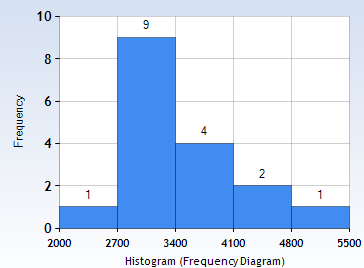
\includegraphics[width=\textwidth]{figure_1.png}
    \caption{Hisogram kolejnych wywołań (monitory), milisekundy}
\end{figure}

Średnia uzyskanych wartości to 3405 ms.

Poniżej eksperyment z takimi samymi parametrami, ale przy użyciu klasy \textit{Lock} z \textit{Java Concurrency Utilities}:

\begin{figure}[H]
    \centering
    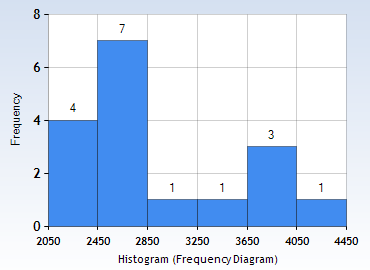
\includegraphics[width=\textwidth]{figure_2.png}
    \caption{Hisogram kolejnych wywołań (\textit{Java Concurrency Utilities}), milisekundy}
\end{figure}

Średnia uzyskanych wartości to 2918 ms, jest mniejsza niż w przypadku użycia monitorów.
Zwiększanie wartości $M$ skutkuje liniowym wzrostem czasu trwania wykonywania programu.
Gdy użyte zostają wartości $n \neq m$, program zbyt często się blokuje.

\section{Wnioski}

Użycie narzędzi z pakietu \textit{Java Concurrency Utilities} pozwala na osiągnięcie tego
samego rezultatu,co przy używaniu monitorów i funkcji \textit{wait} oraz \textit{notifyAll}
, jednak dużo łatwiej oraz często optymalniej. Pakiet udostępnia również narzędzia do
przydatne w wielu konkretnych scenariuszach, np. \textit{AtomicInteger}, odpowiednik
typu \textit{int} zapewniający atomowość operacj.

\section{Bibliografia}

\begin{enumerate}
    \item 
    Dokumentacja języka Java - docs.oracle.com
\end{enumerate}


\end{document}